\problem{}
Consider an $n \times n$ grid graph $G$, as shown below.

\begin{figure}[h]
    \centering
    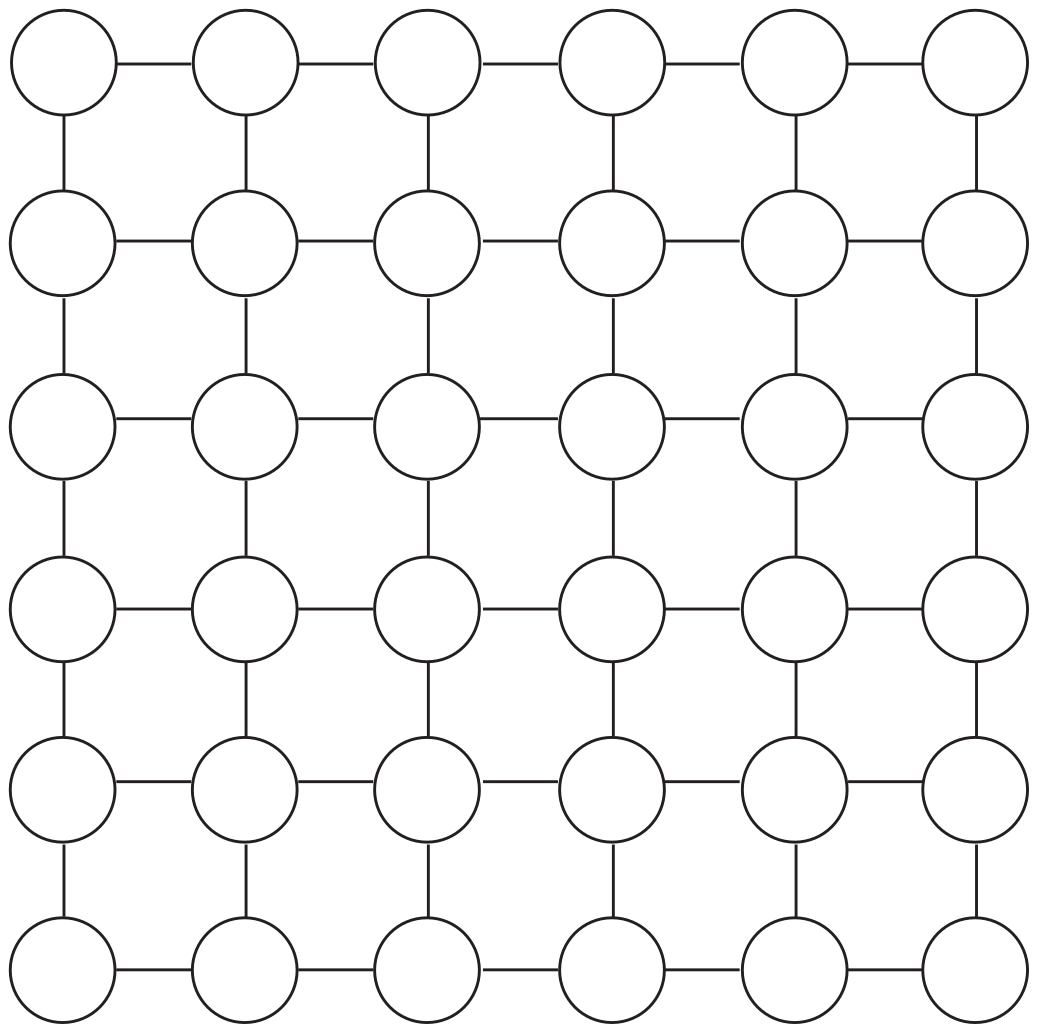
\includegraphics[width=0.4\linewidth]{media/p4.png}
\end{figure}

Each node $v$ in $G$ has a weight $w(v) > 0$.  You want to choose an independent set of nodes with maximum total weight.  That is, you want to choose a set of nodes $S$ with maximum total weight such that for any $v \in S$, none of $v$'s neighbors are in $S$.  To do this, consider the following greedy algorithm.  Let $V$ be the set of all nodes in $G$.  Choose the node in $V$ with the largest weight (breaking ties arbitrarily), add it to the independent set, then remove the node and all its neighbors from $V$.  Repeat this process until $V$ is empty.  Let $S$ be the output of this algorithm.   Solve the following problems.

\begin{enumerate}
\item Let $T$ be any independent set in $G$.  Show that for each node $v \in T$, either $v \in S$, or there is a neighbor $v'$ of $v$ with $v' \in S$ and $w(v) \leq w(v')$.
\item Show that the greedy algorithm is a 4-approximation.
\end{enumerate}


\vspace{5mm}

\solution{}
1.







2.







